\documentclass{beamer}
\usetheme{Madrid}
\usepackage{tikz}
\usepackage{graphicx}
\usepackage{subcaption}
\usepackage{xcolor,colortbl}
\usepackage{pgfplots}
\usepackage{bchart}
\usetikzlibrary{shapes}
\usepackage[font = small, skip = 0pt]{caption}

\tikzstyle{golla} = [circle,draw]
\tikzstyle{box} = [rectangle,draw, text centered]
\tikzstyle{oval} = [ellipse,draw, text centered]
\definecolor{Gray}{gray}{0.85}
\definecolor{LightCyan}{rgb}{67, 250, 243}


\title[\#MeToo]{Can Women Break the Glass Ceiling?: An Analysis of \#MeToo Hashtagged Posts on Twitter}
\author[BUET]{Naeemul Hassan\\Manash Kumar Mandal\\Mansurul Bhuiyan\\Aparna Moitra\\Syed Ishtiaque Ahmed}

\date{\today}


\begin{document}
	\maketitle
	\begin{frame}
	\centering
		\textbf{Presented By :} \\Adiba Shaira (1605097)\\
		 Muntaka Ibnath (1605106)\\ Meher Afroz Sworna (1605114)
	\end{frame}
	
	\begin{frame}{Table of Contents}
		\tableofcontents
	\end{frame}
	\section{Introduction}
	\begin{frame}
		\frametitle{Introduction}
		\begin{itemize}
			\item October 15, 2017 : Tweeter news feed exploded by a tweet  of Alyssa Milano  \pause
			\item More than 4.5 million posts within 24 hours
			
		\end{itemize}
	\end{frame}
	\section{Previous Works}
	\begin{frame}
		\frametitle{Previous Works}
		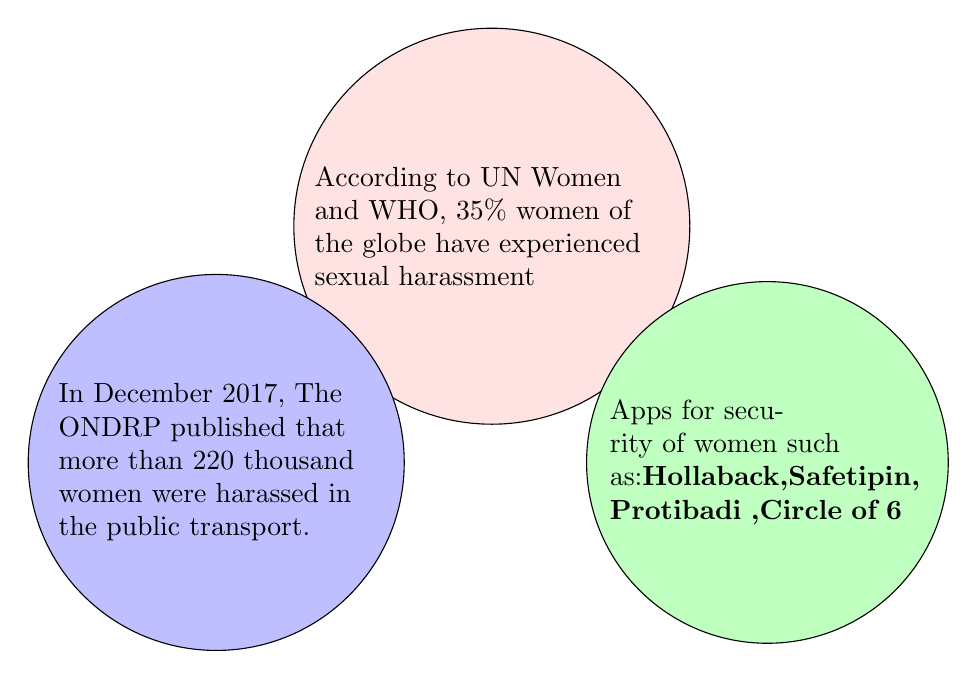
\begin{tikzpicture}
		\centering
		\node[golla,fill = pink!45, text width=4.5cm] at(6.5,3.8)(point1) {According to UN Women and WHO, 35\% women of the globe have experienced sexual harassment};\pause
		\node[golla,fill=blue!25,text width=4cm]at(3,0.8)(point2){In December 2017, The ONDRP published that more than 220 thousand women were harassed in the public transport.};\pause
		\node[golla,fill=green!25,text width=4cm]at(10,0.8)(point3){Apps for security of women such as:\textbf{Hollaback,Safetipin, Protibadi
			,Circle of 6}};
		
		\end{tikzpicture}
		
	\end{frame}
	\section{Data Collection}
	\begin{frame}
		\frametitle{Data Collection}
		\centering
		\begin{tabular}{|l|l|l|l|l|}
			\hline
			\rowcolor{LightCyan}
			\textbf{City} & \textbf{\#Tweets} & \textbf{Male} & \textbf{Female} & \textbf{Female(\%)}   \\
			
			\hline
			Dallas & 1249 & 144 & 471 & 76.59 \\
			\hline
			Dhaka & 82 & 32 &  22 & 40.74  \\
			\hline
			Indianapolis & 1203 & 180 & 452 & 71.52  \\
			\hline
			Kansan City & 448 & 61 & 208 & 77.32  \\
			\hline
			Karachi & 250 & 44 & 55 & 55.56  \\
			\hline
			Mumbai & 2778 & 724 & 674 & 48.21  \\
			\hline
			New York & 1878 & 267 & 754 & 73.85  \\
			\hline
			North Dakota & 110 & 18 & 34 & 65.38  \\
			\hline
			Portland & 849 & 146 & 316 & 68.4  \\
			\hline
			Saint Louis & 619 & 92 & 224 & 70.89  \\
			\hline
			Tehran & 114 & 13 & 32 & 71.11  \\
			\hline
			
			
		\end{tabular}
		
	\end{frame}
	\section{Age and Gender Distribution}
	\begin{frame}
		\frametitle{Analysis}
		\begin{itemize}
			\item \textbf{Age and Gender Distribution}\pause
		\end{itemize}
		\begin{figure}[h]
			\centering
			\begin{subfigure}{0.45\textwidth}
				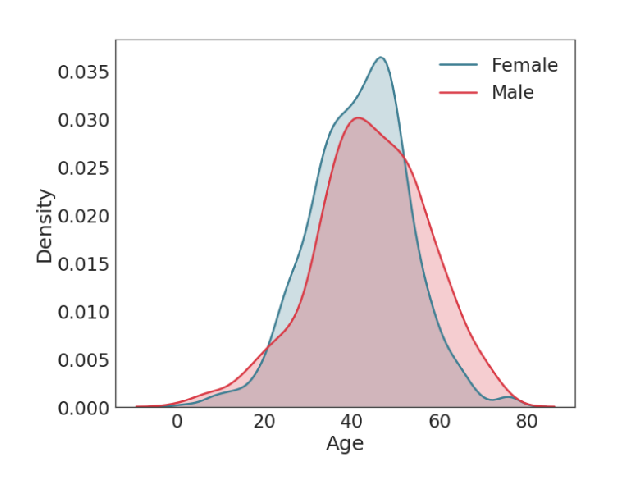
\includegraphics[width=0.85\textwidth]{SS1}
				%\includegraphics[width=0.85\textwidth]{p1.png}
				\caption{US}
			\end{subfigure} \pause
			~
			\begin{subfigure}{0.45\textwidth}
				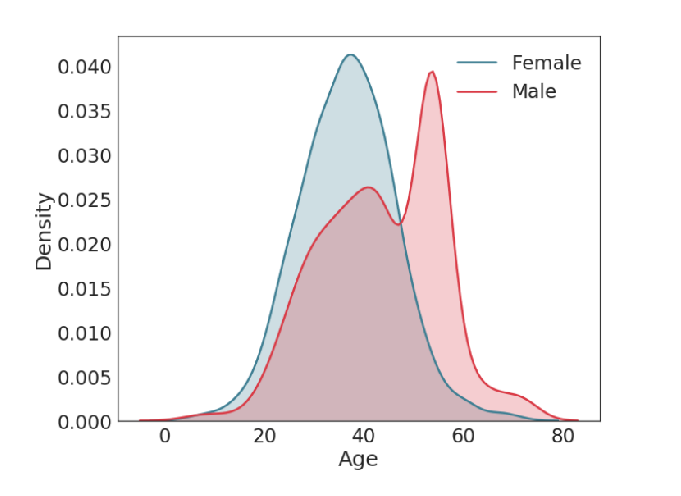
\includegraphics[width=0.85\textwidth]{SS2}
				\caption{Asia}
			\end{subfigure}
			\caption{Age distribution of female and male users}
		\end{figure}
		
	\end{frame}
\begin{frame}
\frametitle{Harassment Claims in a Particular Form}

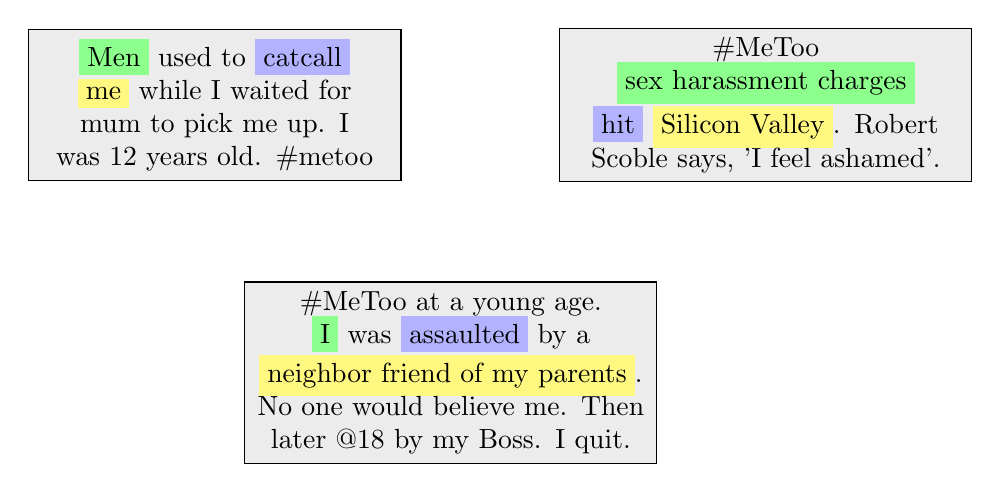
\begin{tikzpicture}
\node[box,fill=gray!15, text width=4.5cm] at(3,2.5)(rec1) {
	\colorbox{green!45}{Men} used to \colorbox{blue!30}{catcall} 
	\colorbox{yellow!50}{me} while I waited for mum to pick me up. I was 12 years old. \#metoo};\pause
\node[box,fill=gray!15,text width=5cm, below of=rec1]at(6,0.1)(rec2){\#MeToo at a young age. \colorbox{green!45}{I} was 
	\colorbox{blue!30}{assaulted} by a \colorbox{yellow!50}{neighbor friend of my parents}. No one would believe me. Then later @18 by my Boss. I quit.};\pause
\node[box,fill=gray!15,text width=5cm]at(10,2.5)(rec3){\#MeToo 
	\colorbox{green!45}{sex harassment charges} \colorbox{blue!30}{hit}
	\colorbox{yellow!50}{Silicon Valley}. Robert Scoble says, 'I feel ashamed'.};
\end{tikzpicture}
\end{frame}


	
	
	
	\section{Category and Role Analysis}
	\begin{frame}
		\frametitle{Harassment Categories}
		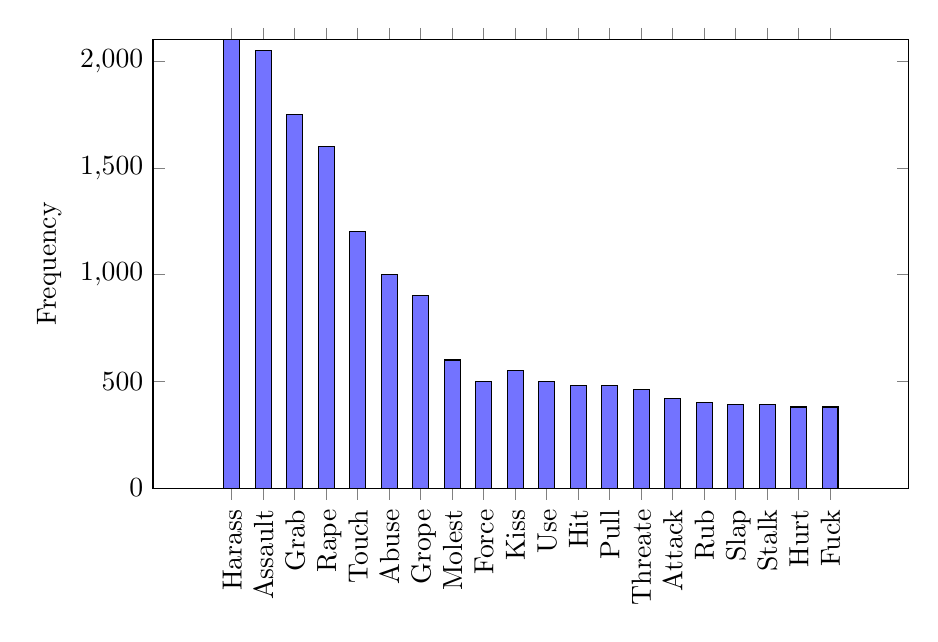
\begin{tikzpicture}
		\begin{axis}[
		ybar,
		bar width=.2cm, % Width of the bar
		x=.4cm, % Distance between the centers of the bars
		enlarge x limits={abs=1cm}, % The distance between the center of the first bar and the left edge
		enlarge y limits=false,
		ymin=0,
		xtick=data,
		xlabel=,
		symbolic x coords={Harass, Assault, Grab,Rape,Touch,Abuse,Grope,Molest,Force,Kiss,Use,Hit,Pull,
			Threate,Attack,Rub,Slap,Stalk,Hurt,Fuck},
		xtick=data,
		ylabel=Frequency,
		xticklabel style={text height=0ex},
		xticklabel style={rotate=90,anchor=north east},
		%ymajorgrids,yminorgrids,minor y tick num=4,
		]
		
		
		\addplot[ybar,fill=blue!55] coordinates {
			(Harass,2100)(Assault,  2050)
			(Grab,1750)(Rape,1600)(Touch,1200)(Abuse,1000)
			(Grope,900)(Molest,600)(Force,500)(Kiss,550)
			(Use,500)(Hit,480)(Pull,480)(Threate,460)(Attack,420)
			(Rub,400)(Slap,390)(Stalk,390)(Hurt,380)(Fuck,380)
		};
		
		
		\end{axis}
		
		
		\end{tikzpicture}
	\end{frame}




	\begin{frame}
		\frametitle{Frequency of Harasser Roles}
		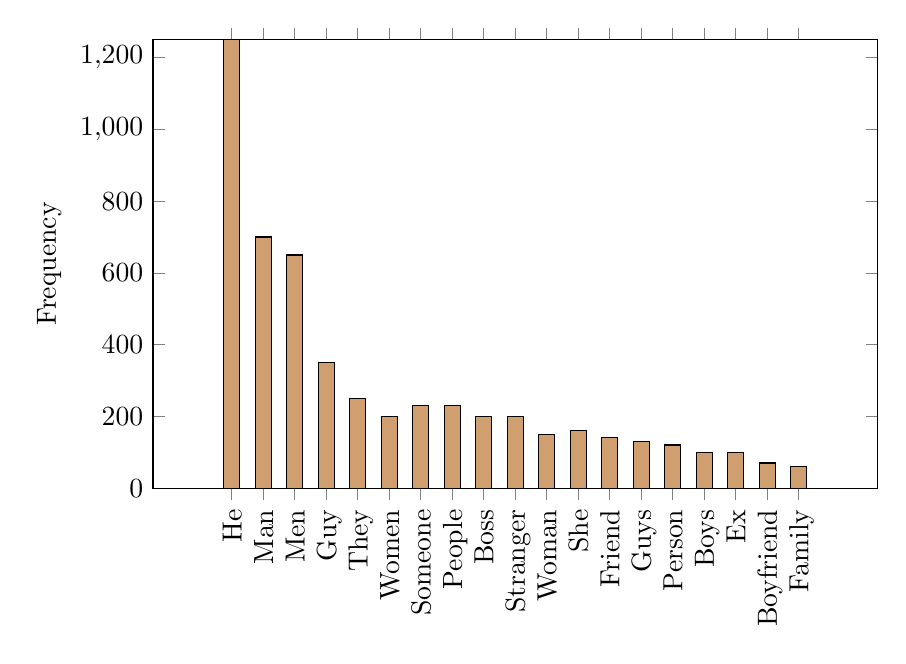
\begin{tikzpicture}
		\begin{axis}[
		ybar,
		bar width=.2cm, % Width of the bar
		x=.4cm, % Distance between the centers of the bars
		enlarge x limits={abs=1cm}, % The distance between the center of the first bar and the left edge
		enlarge y limits=false,
		ymin=0,
		xtick=data,
		xlabel=,
		symbolic x coords={He,Man,Men,Guy,They,Women,Someone,People,Boss,Stranger,Woman,She,Friend,Guys,Person,Boys,Ex,Boyfriend,Family},
		xtick=data,
		ylabel=Frequency,
		xticklabel style={text height=0ex},
		xticklabel style={rotate=90,anchor=north east},
		%ymajorgrids,yminorgrids,minor y tick num=4,
		]
		
		
		\addplot[ybar,fill=brown!75] coordinates {
			(He,1250)(Man,700)(Men,650)(Guy,350)(They,250)(Women,200)(Someone,230)(People,230)(Boss,200)(Stranger,200)(Woman,150)
			(She,160)(Friend,140)(Guys,130)(Person,120)(Boys,100)(Ex,100)(Boyfriend,70)(Family,60)
		};
		
		
		\end{axis}
		
		
		\end{tikzpicture}
	\end{frame}


\begin{frame}
	\frametitle{Frequency in Different Regions}
	\begin{figure}[h]
		\centering
		\begin{subfigure}{0.35\textwidth}
			\includegraphics[width=0.85\textwidth,height=2.7cm,width=3.3cm]{usa.eps}
		\end{subfigure}
		~
		\begin{subfigure}{0.35\textwidth}
			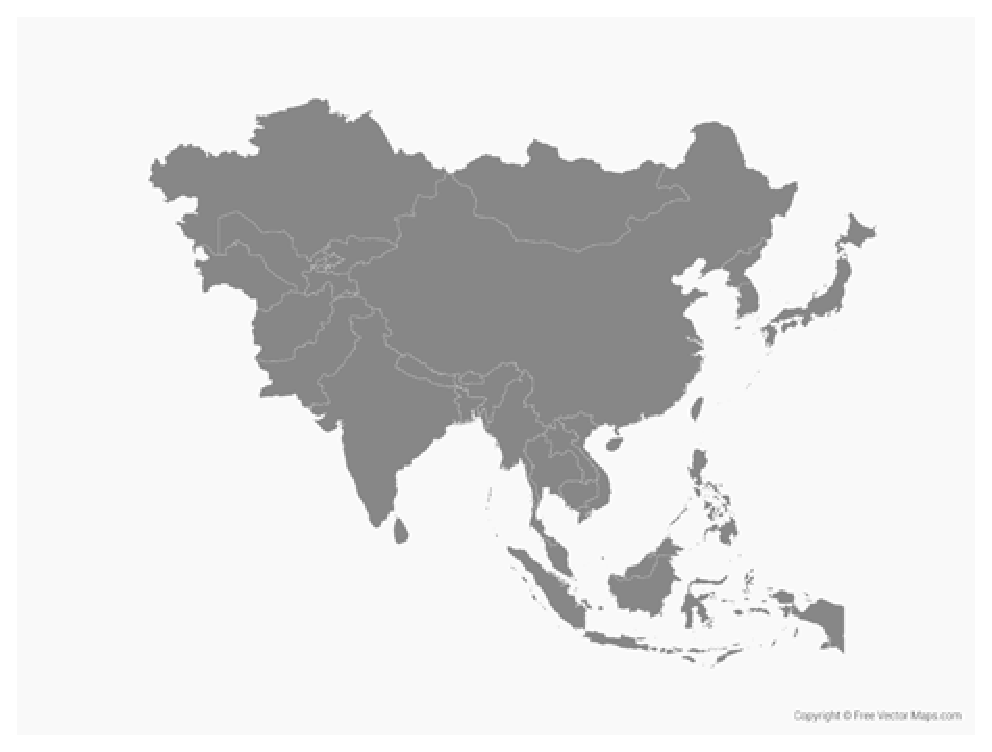
\includegraphics[width=0.85\textwidth,height=2.5cm,width=3.3cm]{asia.eps}
		\end{subfigure}
		
		\begin{subfigure}{0.4\textwidth}
			\includegraphics[width=0.85\textwidth,height=4cm]{US.eps}
			\centering
			\caption{USA}
		\end{subfigure}
	~
		\begin{subfigure}{0.4\textwidth}
			\includegraphics[width=0.85\textwidth,height=3.5cm]{Asia.eps}
			\centering
			\caption{Asia}
		\end{subfigure}   
	\caption{Top 10 harassment categories in different regions}     
	\end{figure}
	
	
\end{frame}
	\section{Topic Distribution}
	\begin{frame}
		\frametitle{Topic Distribution}
		Relevance of a word with respect to a topic,$r(w, k)$, is calculated using the following equation :
			\begin{block}{Equation}
				\begin{equation*}
				r(w,k) = \lambda * \log(\sigma_{kw}) + (1 - \lambda)*\log\left(\frac{\sigma_{kw}}{P_w}\right)
				\end{equation*}
				Here ,\\ $\sigma_{kw} = $  The probability of word $w$ for topic $k$ \\ $P_w = $The marginal probability of term $w$ in the whole dataset\\$\lambda = $ Tuning parameter
			\end{block}
		
	\end{frame}

	\begin{frame}
		\frametitle{Dataset(1)}
		\begin{figure}[h]
			\centering
			\begin{subfigure}{0.45\textwidth}
				
\includegraphics[width=0.8\textwidth]{SS61.eps}
				\centering
				\caption{Recognition}
			\end{subfigure}\pause
			~
			\begin{subfigure}{0.45\textwidth}
				
\includegraphics[width=0.8\textwidth]{SS62.eps}
				\centering
				\caption{Weinstein Effect}
			\end{subfigure}\pause
		
			\begin{subfigure}{0.45\textwidth}
				
\includegraphics[width=0.8\textwidth]{SS63.eps}
				\centering
				\caption{Advertisement}
			\end{subfigure}
		\end{figure}
	\end{frame}
	\begin{frame}
	\frametitle{Dataset(2)}
		\begin{figure}[h]
			\centering
			\begin{subfigure}{0.45\textwidth}
				
\includegraphics[width=0.8\textwidth]{SS64.eps}
				\centering
				\caption{Nature and Location}
			\end{subfigure}\pause
			~
			\begin{subfigure}{0.45\textwidth}
				
\includegraphics[width=0.8\textwidth]{SS65.eps}
				\centering
				\caption{Young Victims}
			\end{subfigure}\pause
		
			\begin{subfigure}{0.45\textwidth}
				
\includegraphics[width=0.8\textwidth]{SS66.eps}
				\centering
				\caption{Media Coverage}
			\end{subfigure}
		\end{figure}
	\end{frame}
	\section{Psychological Constructs}
	\begin{frame}
		\frametitle{Psychological Constructs Analysis}
		\begin{figure}
			\centering
			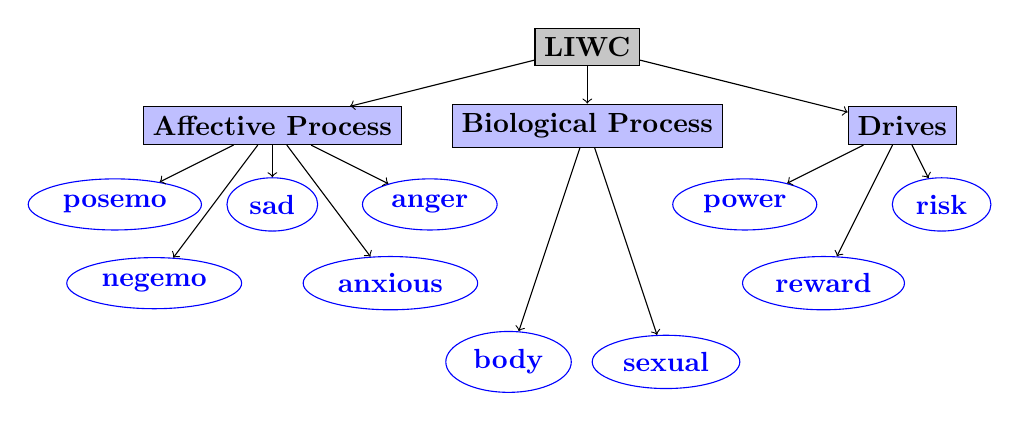
\begin{tikzpicture}
			\centering
			\node[box,fill = gray!45](liwc){\textbf{LIWC}};\pause
			\node[box, below of=liwc, xshift = -4cm, fill = blue!25](ap){\textbf{Affective Process}};
			\draw[->] (liwc) -- (ap);\pause
			\node[box, below of=liwc, fill = blue!25](bp){\textbf{Biological Process}};
			\draw[->] (liwc) -- (bp);\pause
			\node[box, below of=liwc, xshift = 4cm,fill = blue!25](dr){\textbf{Drives}};
			\draw[->] (liwc) -- (dr);\pause
			\node[oval, below of=ap, xshift = -2cm,blue](pos){\textbf{posemo}};
			\draw[->] (ap) -- (pos);\pause
			\node[oval, below of=ap, xshift = -1.5cm, yshift = -1cm,blue](neg){\textbf{negemo}};
			\draw[->] (ap) -- (neg);\pause
			\node[oval, below of=ap,blue](sad){\textbf{sad}};
			\draw[->] (ap) -- (sad);\pause
			\node[oval, below of=ap, xshift = 1.5cm,yshift = -1cm,blue](anxious){\textbf{anxious}};
			\draw[->] (ap) -- (anxious);\pause
			\node[oval, below of=ap,xshift = 2cm,blue](ang){\textbf{anger}};
			\draw[->] (ap) -- (ang);\pause
			\node[oval, below of=bp, xshift = -1cm,yshift=-2cm,blue](body){\textbf{body}};
			\draw[->] (bp) -- (body);\pause
			\node[oval, below of=bp, xshift = 1cm,yshift=-2cm,blue](sexual){\textbf{sexual}};
			\draw[->] (bp) -- (sexual);\pause
			\node[oval, below of=dr, xshift = -2cm,blue](power){\textbf{power}};
			\draw[->] (dr) -- (power);\pause
			\node[oval, below of=dr,xshift=-1cm,yshift=-1cm,blue](reward){\textbf{reward}};
			\draw[->] (dr) -- (reward);\pause
			\node[oval, below of=dr, xshift = 0.5cm,blue](risk){\textbf{risk}};
			\draw[->] (dr) -- (risk);
			\end{tikzpicture}
		\end{figure}
	\end{frame}
	\begin{frame}
		\frametitle{LIWC Term Distribution in Asia}
		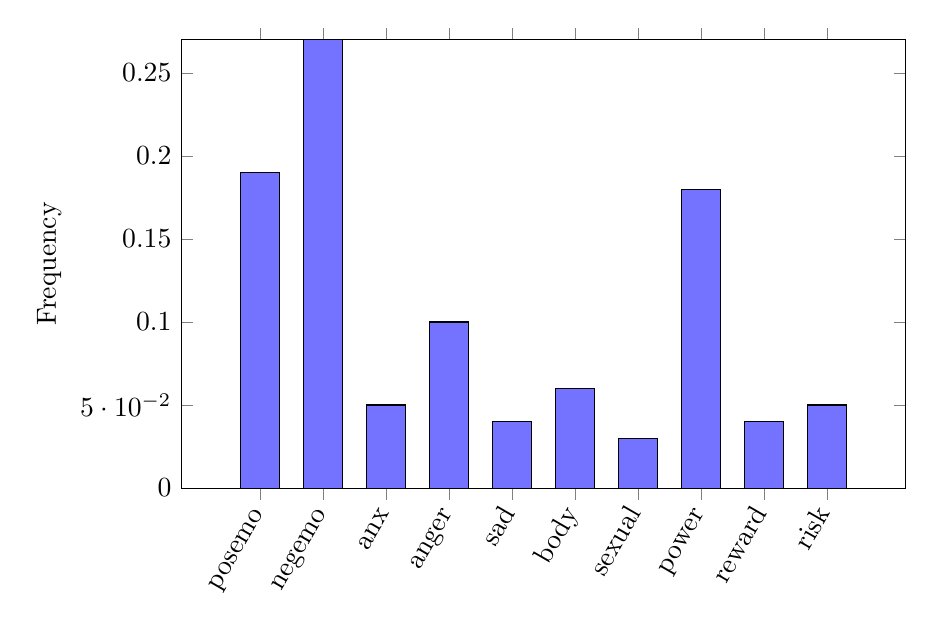
\begin{tikzpicture}
		\begin{axis}[ybar,bar width=0.5cm,x=0.8cm,enlarge x limits = {abs=1cm},enlarge y limits=false,ymin=0,
		xtick=data,
		symbolic x coords={posemo, negemo, anx, anger, sad, body, sexual, power, reward, risk},xtick=data,ylabel=Frequency,xticklabel style={text height=0ex},
		xticklabel style={rotate=60,anchor=north east}
		]
		
		\addplot[ybar,fill=blue!55] coordinates { (posemo,0.19) (negemo,0.27) (anx,0.05) (anger,0.1)(sad,0.04)(body,0.06)(sexual,0.03)(power,0.18)(reward,0.04)(risk,0.05)};
		
		\end{axis}
		
		\end{tikzpicture}
	\end{frame}
	\section{Limitations}
	\begin{frame}
		\frametitle{Limitations}
		\begin{itemize}
			\item Findings may not be generalized \pause
			\item Not the representation of the whole movement \pause
			\item Misrepresentation on social media
		\end{itemize}
	\end{frame}
\section{Conclusion}
\begin{frame}
\frametitle{Conclusion}
\begin{figure}
	\centering
	\begin{subfigure}{0.45\textwidth}
		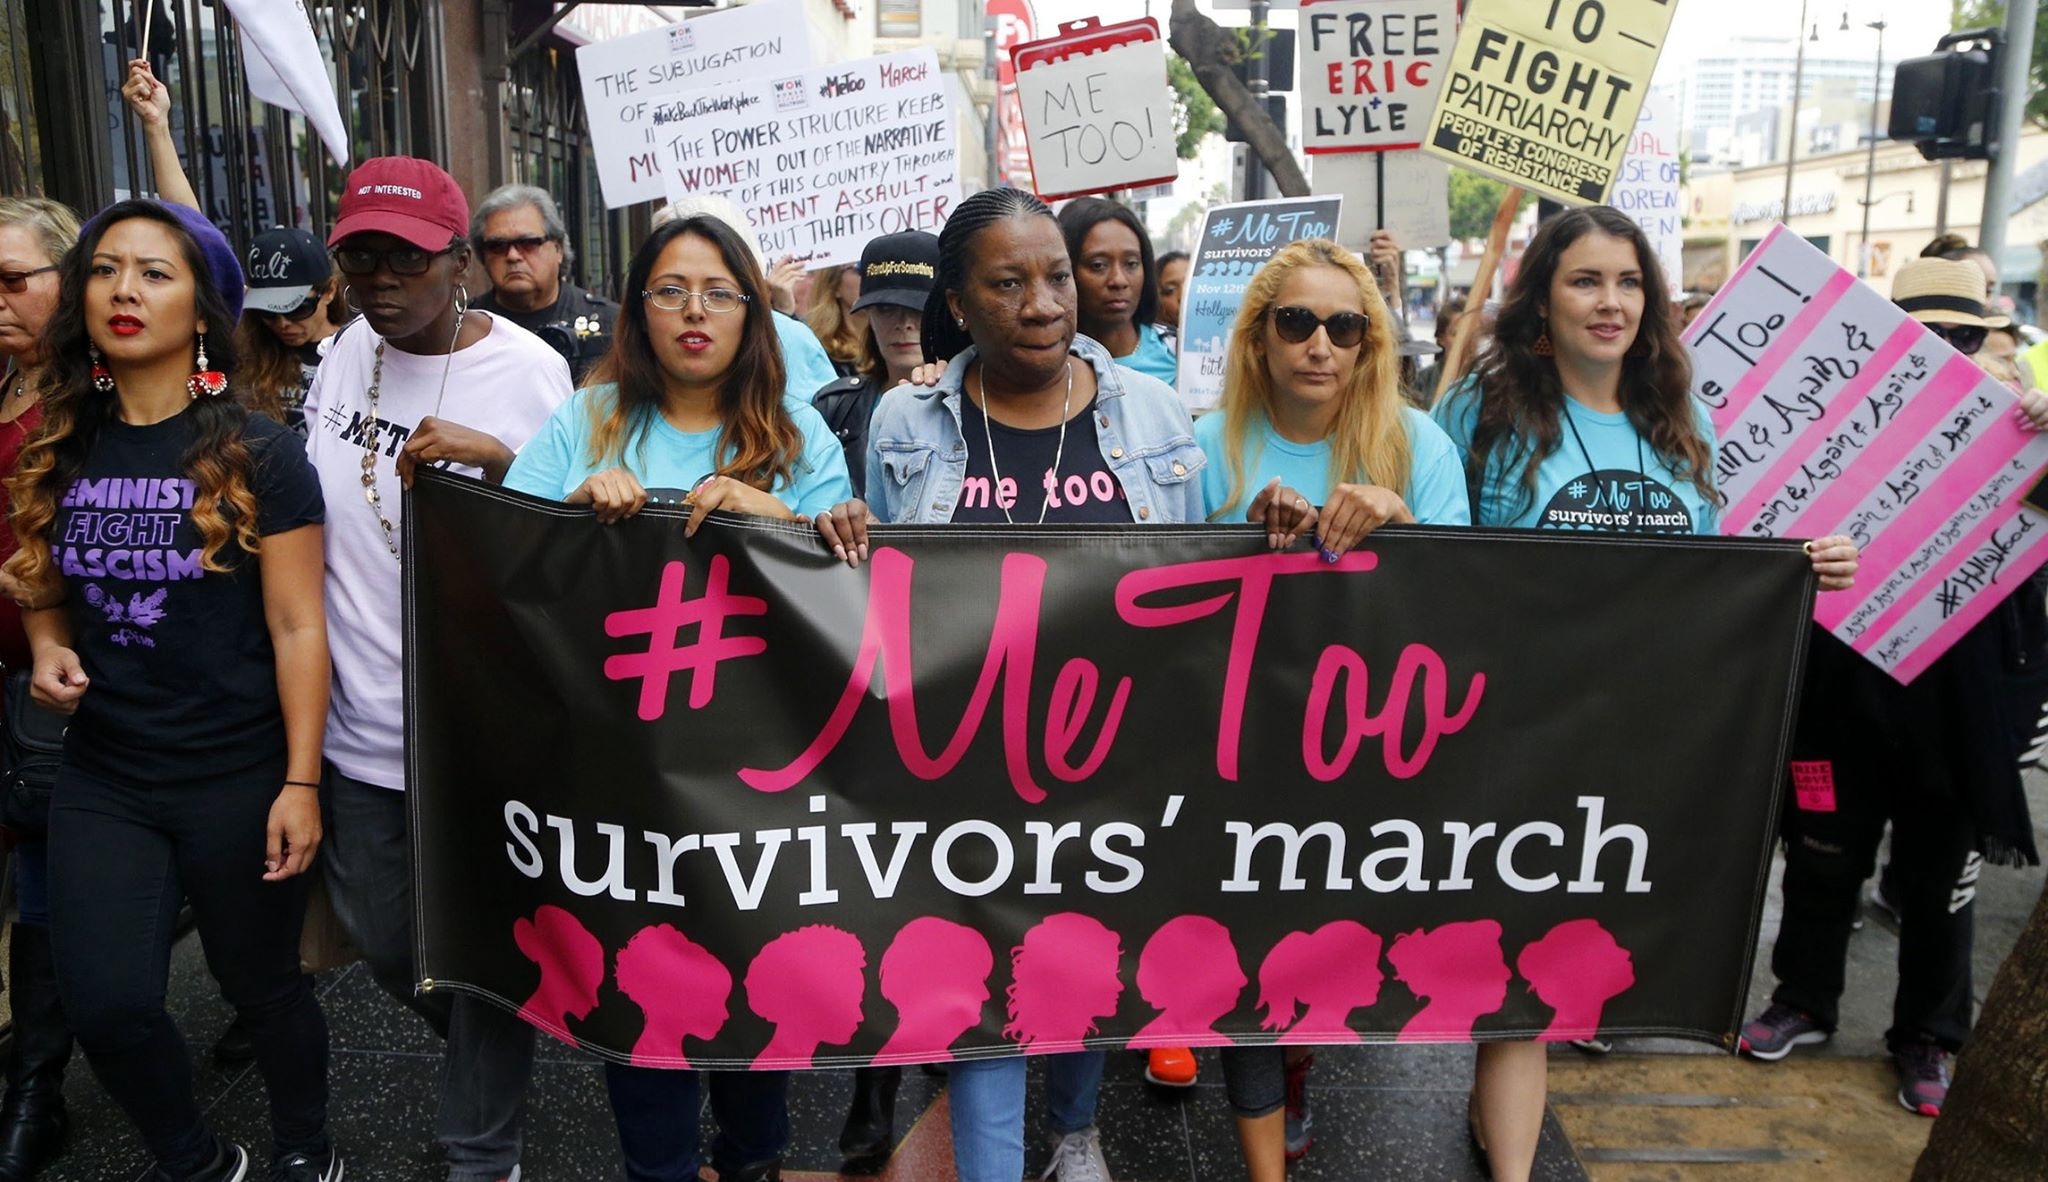
\includegraphics[width=0.95\textwidth]{pic1.jpg}
	\end{subfigure}
	~
	\begin{subfigure}{0.45\textwidth}
		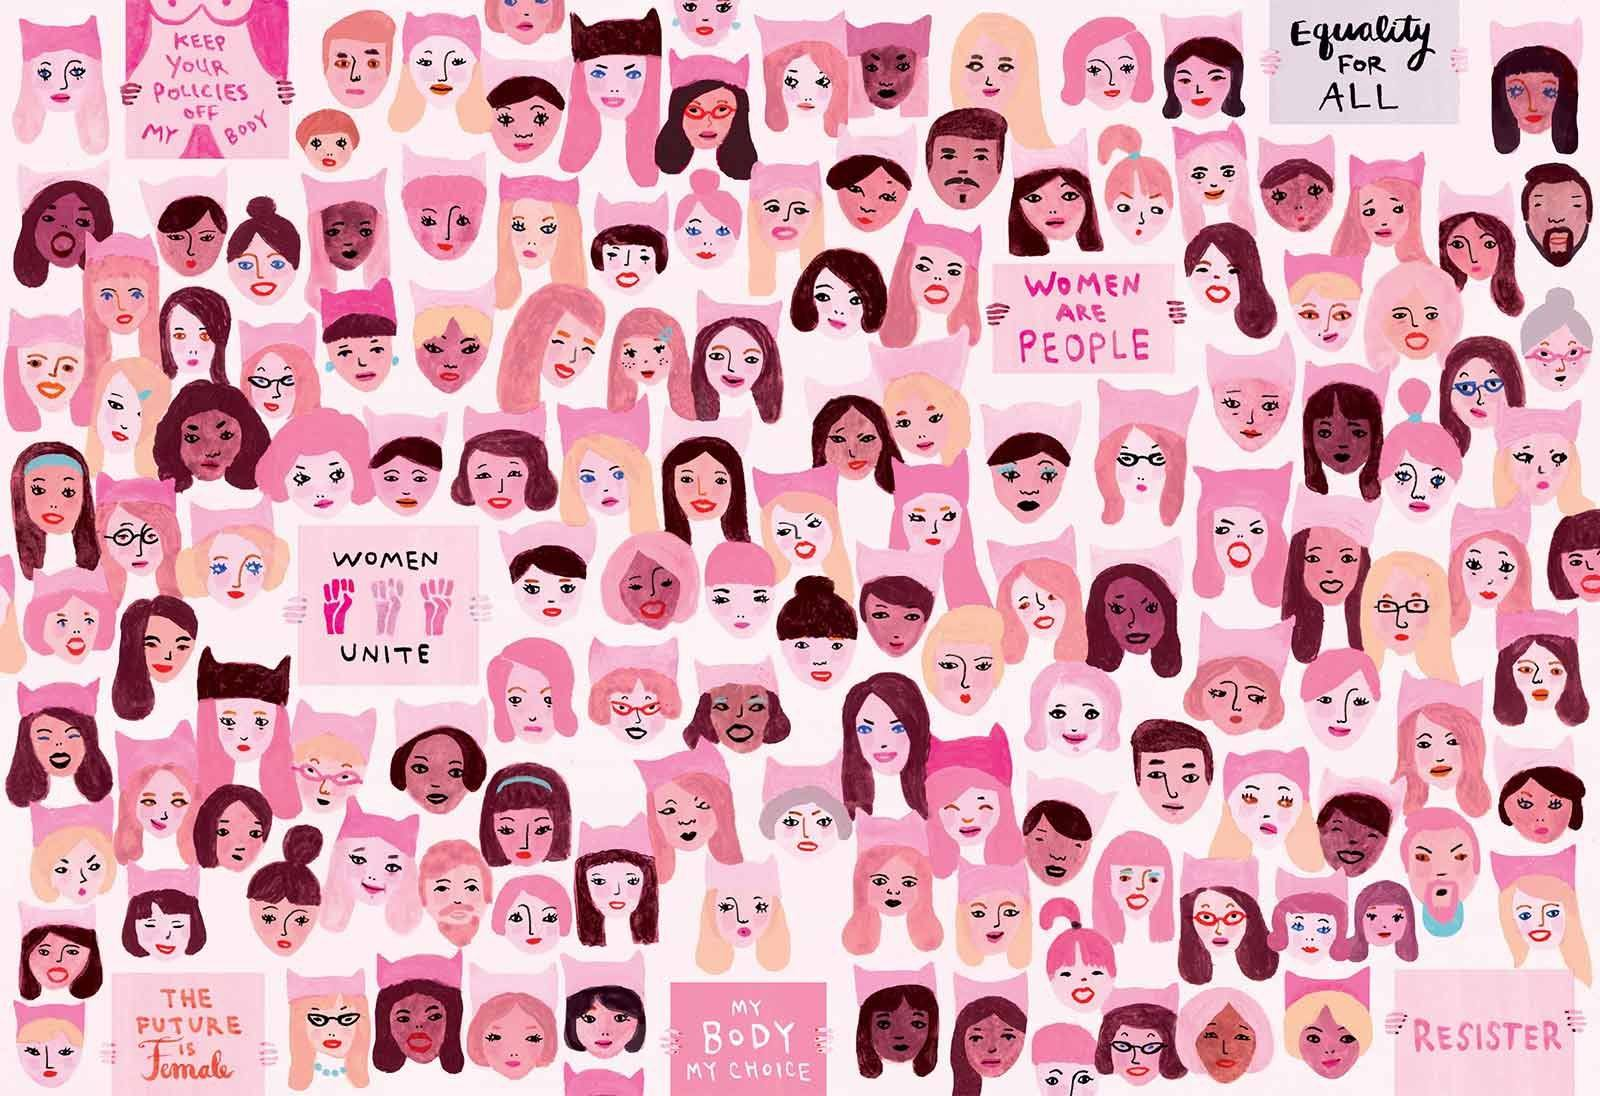
\includegraphics[width=0.95\textwidth]{pic2.jpg}
	\end{subfigure}
	\caption{\#MeToo Movement}
	
\end{figure}

\end{frame}
\begin{frame}
\centering
	\textbf{\Huge Thank You}
\end{frame}
\end{document}